\section{Introduction}

Software development requires the ability to think about several
dimensions simultaneously. For large programs, writing the actual
instructions for the computer is not as difficult as figuring out the
details of what the computer is supposed to do. After analyzing what is
needed, program design brings together the data structures, algorithms,
objects, and interactions that accomplish the required tasks. Despite
the importance of analysis and design, programming is still the central
act of software development for several reasons. The weak form of the
\index{Sapir-Whorf}Sapir-Whorf hypothesis suggests that the programming
language we use steers and guides the way we think about software, so
it affects our designs. Software designs are mathematical theorems,
while programs are the proofs that test those designs. As in other
branches of mathematics, the proofs reign supreme. In addition, a
correct design can be foiled by an inferior implementation.

This book is a programmer{\textquotesingle}s guide for an exciting
programming language called Unicon that has something to offer both
computer scientists as well as casual programmers. In this book you
will find explanations of fundamental principles, unique language
idioms, and advanced concepts and examples. Unicon exists within the
broader context of \ software development, so we also cover practical
software engineering fundamentals. We view writing a correct, working
program as the central task of software engineering. This does not
happen as an automatic consequence of the software design process. Make
no mistake: if you program very much, the programming language you use
is of vital importance. If it weren{\textquotesingle}t, we would still
be programming in machine language.

\subsection{Prototyping and the Spiral Model of Development}

A software \index{prototype}prototype is a working subset of a software
system. Prototypes are used to check software designs and user
interfaces, to demonstrate key features to customers, or to prove the
feasibility of a proposed solution. A prototype may help generate
customer feedback on missing functionality, provide insight on how to
improve the design, lead to a decision about whether to go ahead with a
project or not, or form a starting point for the algorithms and data
structures that will go into the final product. Prototyping is done
early in the software development process. It fits naturally into the
\index{spiral model}\textit{spiral model} of development proposed by
\index{Boehm, Barry}Barry Boehm (1988). Figure I-1 shows the spiral
model; time is measured by the distance from the center. Analysis,
design, coding, and evaluation are repeated to produce a better product
with each iteration. {\textquotedbl}Prototyping{\textquotedbl} is the
act of coding during those iterations when the software is not yet
fully specified or the program does not yet even remotely implement the
required functionality.

\begin{center}
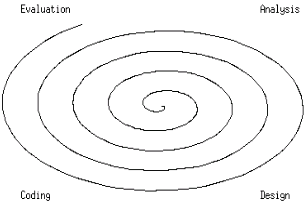
\includegraphics[width=2.5402in,height=1.6799in]{ub-img/ub-img4.png}
\end{center}

{\sffamily\bfseries Figure I-1}
{\sffamily The Spiral Model of Software Development}

\bigskip

\textit{Tight} spirals are better than loose spirals. The more powerful
the prototyping tools, the less time and money expended in early
iterations of development. This savings translates into either faster
time to market, or a higher quality product. Some prototypes are thrown
away once they have served the purpose of clarifying requirements or
demonstrating a technique to be used. This is OK, but a prototype that
is gradually enhanced until it becomes the final production system is
more consistent with the spiral model.

\subsection{Icon: a Very High Level Language for Applications}

Icon is a \index{very high-level language}very high-level language that
originated at the University of Arizona. It is ideal for prototyping a
wide range of applications. Icon benefits from the experience that its
inventors gained from designing, implementing, and supporting a user
community for an earlier very high-level language,
\index{SNOBOL4}SNOBOL4. Icon incorporates seminal research
contributions to the field of programming languages. We love Icon not
because it embodies neat research, but because it is more fun and
easier to program in than other languages. Unlike most very high-level
languages, which revel in cryptic syntax, Icon{\textquotesingle}s
syntax is not just more powerful, but in many cases more
\textit{readable} than the other programming languages of today. This
gain in expressive power without sacrificing readability is an
astonishing and addicting result of Icon{\textquotesingle}s elegant
design.

The current version of Arizona Icon is version 9.5. It is described in
\textit{The Icon Programming Language}, \textit{3rd edition} by Ralph
and Madge Griswold (1996). The \ reference implementation of Icon is a
virtual machine interpreter. The language evolved through many releases
over two decades and is far more capable than it was originally. For
example, Icon now includes portable high-level graphics facilities
described in the book \textit{Graphics Programming in Icon}, by Ralph
\index{Griswold, Ralph}Griswold, Clinton Jeffery, and Gregg
\index{Townsend, Gregg}Townsend (1998). Icon is mature, and its
designers do not envision major additions to the language at this
point. Over the past decade many people have worked to increase
Icon{\textquotesingle}s suitability for a wide range of applications.
At the University of Arizona, examples of this work have included
implementations of Icon that generate C (which is compiled to native
machine code for speed), and \index{Java virtual machine}Java virtual
machine code (for portability).

\subsection{Enter Unicon: More Icon than Icon}

The name Unicon\textbf{\textsuperscript{ }}refers to the descendant of
Icon described in this book and distributed from unicon.org. Unicon is
Icon with the authors{\textquotesingle} additions: elegant, portable,
and platform-independent facilities that have become ubiquitous in
applications development, such as objects, networks, and databases.
Unicon is created from the same public domain source code that Arizona
Icon uses, so it has a high degree of compatibility. We
didn{\textquotesingle}t feel free to call it version 10 of the Icon
language, since it is not produced or endorsed by the Icon Project at
the University of Arizona. They are not responsible for
Unicon{\textquotesingle}s bugs, nor does it make their standard release
of Icon out of date.

Just as the name Unicon frees the Icon Project of all responsibility for
our efforts, it frees us from the requirement of backward
compatibility. While Unicon is 99.9 percent backward compatible (this
measurement is figurative, not literal) with Icon, dropping 0.1 percent
compatibility allows us to clear out some dead wood and more
importantly, to make some improvements in the operators that will
benefit everyone at the expense of...no one but the compatibility
police.

This book covers the features of Icon and Unicon together. A
compatibility check list and description of the differences between
Icon and Unicon are given in Appendix D.

\subsection{The Programming Languages Food Chain}

It is interesting to compare Icon and Unicon with the competition. One
kind of competition comes from mainstream systems programming languages
such as C, C++, and \index{Java}Java. Like the assembler languages that
comprised the mainstream before them, these languages are ideal tools
for writing all sorts of programs, so long as vast amounts of
programmer time are available. The computing culture has long
understood that throwing more programmers at a big project is a poor
solution, and programmers are getting more expensive while computing
resources continue to become cheaper. These pressures slowly but
inexorably lead to the use of higher-level languages and the
development of better design tools and development methods. Such human
changes are incredibly slow compared to technological changes, but they
are visibly taking place nevertheless. Today, many of the most
productive programmers are using extra CPU cycles and megabytes of RAM
to make it several times faster to develop useful programs.

There is a subcategory of mainstream languages, marketed as \index{rapid
application development}\textit{rapid application development} (RAD)
languages, whose stated goals seem to address this phenomenon.
Languages such as \index{Visual Basic}Visual Basic,
\index{Delphi}Delphi, and \index{PowerBuilder}PowerBuilder provide
graphical interface builders and integrated database connectivity,
giving productivity increases in the domain of data entry and
presentation. The value added in these products are in their
programming environments, not their languages. The \index{integrated
development environment}integrated development environments and tools
provided with these languages are to be acclaimed and emulated, but
they do not provide productivity gains that are equally relevant to all
application domains. They are only a partial solution to the needs of
complex applications.

Icon is designed to be easier and faster to program than mainstream
languages. The value it adds is in the expressive power of the language
itself, putting it in the category of {\textquotedbl}very high level
languages.{\textquotedbl} This category includes \index{Lisp}Lisp,
\index{APL}APL, \index{Smalltalk}Smalltalk, \index{REXX}REXX,
\index{Perl}Perl, \index{Tcl}Tcl, and \index{Python}Python; there are
many others. Very high-level languages may be further subdivided into
\index{scripting languages}scripting languages and applications
languages. Scripting languages are generally designed to glue programs
together from disparate sources. They are typically strong in areas
such as multilingual interfacing and file system interactions, while
suffering from weaker expression semantics, typing, scope rules, and
control structures than their applications-oriented cousins.
Applications languages typically originate within a particular
application domain and support that domain with special syntax, control
structures, and data types. Since scripting \textit{is} an application
domain, scripting languages can be viewed as just one prominent
subcategory of very high-level languages.

Icon is an applications language; its SNOBOL roots are in text
processing and linguistics. For many application areas, Icon is the
best programming language currently available. Icon programs are
written faster, in less code, than conventional languages such as C or
Java. Icon programs tend to be more readable and maintainable than
similar programs written in other very high-level languages. This makes
Icon particularly well-suited to the aims of \index{literate
programming}\textit{literate programming}; for example, Icon was used
to implement Norman Ramsey{\textquotesingle}s popular literate
programming tool \texttt{noweb} (Ramsey, 1994). Literate programming is
the practice of writing programs and their supporting textual
description together in a single document.

With Unicon, the core contributions of the Icon language become useful
for an even broader range of applications. This book includes numerous
examples that illustrate the range of tasks for which Unicon is well
suited, and these examples are the best evidence we can provide in
support of our argument.

Consider using Unicon when one or more of the following conditions are
true. The more conditions that are true, the more likely you will
benefit from Unicon.

\begin{itemize}
\item Programmer time must be minimized.
\item Maintainable, concise source code is desired.
\item The program includes complex data structures or experimental
algorithms.
\item The program involves text processing and analysis, custom
graphics, data manipulation, network or file system operations, or
interactions among the above application domains.
\item The program must run on several operating systems and have a
nearly identical graphical user interface with little or no source code
differences.
\end{itemize}
Unicon is not the last word in programming. You probably should not use
Unicon if your program has one or more of the following requirements:

\begin{itemize}
\item The fastest possible performance is needed.
\item The program has hard real-time constraints.
\item The program must perform low-level or platform-specific
interactions with the hardware or operating system.
\item The program must utilize substantial libraries written in
lower-level languages such as C, C++, or FORTRAN.
\end{itemize}
Programming languages play a key role in the software development
enterprise. Icon is an exciting very high-level language with a unique
design that reduces programming time without sacrificing readability.
The Unicon language extends Icon with capabilities such as
\index{object-oriented programming}object-oriented programming and
database management that are useful in many programs, especially larger
programs that use the Internet. This book will show you how Unicon
makes complex programming tasks easier. Many examples from a wide range
of application areas serve to demonstrate how to apply and combine
language constructs to solve real-world problems.

It is time to move past the introductions. Prepare to be spoiled with
one of the most hassle-free programming languages
you{\textquotesingle}ll ever use. You may have the same feelings that
early Italian merchants felt when they gave up using Roman numerals and
switched to the Hindu-Arabic number system. {\textquotedbl}This
multiplication stuff isn{\textquotesingle}t that hard
anymore!{\textquotedbl} 
